\section{Projet}
\subsection{Les livrables}
\begin{frame}
    \frametitle{\color{white}Les livrables}
    \begin{block}{Trois livrables demandés}
    	\begin{itemize}
         \item Une étude détaillée d'OpenPGP et de GnuPG.
         \item Une interface graphique permettant de facilité la compréhension et l'utilisation de GnuPG.
         \item Une étude des limites, et une implantation d'une attaque sur les identifiants de clefs PGP.
       \end{itemize} 
    \end{block}
\end{frame}

\begin{frame}
    \frametitle{\color{white}L'interface graphique : GuiPG}
    \begin{block}{Fonctionnalités}
      \begin{itemize}
        \item Gestion d'un trousseau de clefs gpg.
        \item Actions cryptographiques.
        \item Représentation de la toile de confiance.
        \item Visualisation des commandes nécessaire pour chaque actions.
      \end{itemize}
    \end{block}
\end{frame}
\subsection{Propagation de la confiance} % (fold)

\begin{frame}
  \frametitle{\color{white}Validité non définie}
    \begin{block}{}
      Alice n'a pas attribué de confiance aux trois clefs qu'elle a certifié.\\
      La clé non certifié par Alice n'est donc pas valide.
    \end{block}
    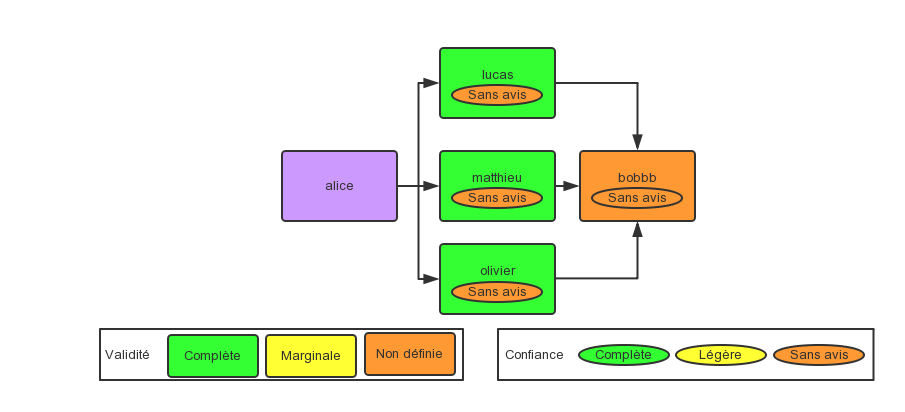
\includegraphics[scale=0.3]{tdcdemoUndefined.png}
\end{frame}
\begin{frame}
  \frametitle{\color{white}Validité Marginal}
    \begin{block}{}
      Une ou deux clef certifié par Alice avec une confiance légère 
      induit une validité marginale sur une clé non certifié par Alice
      mais certifié par les premières.
    \end{block}
    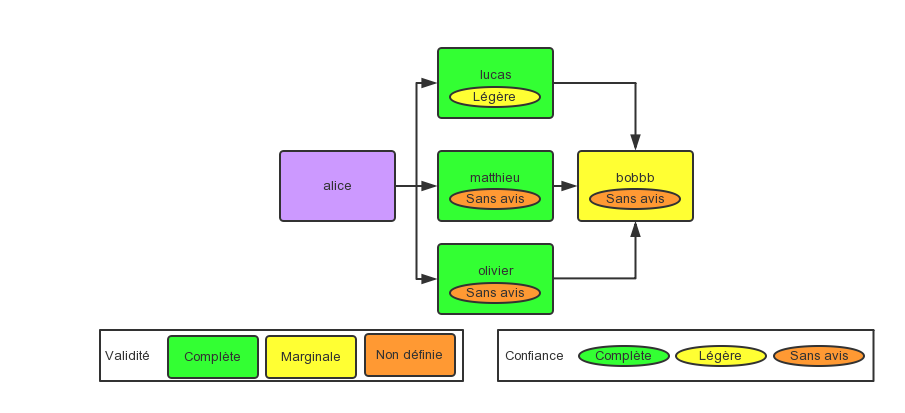
\includegraphics[scale=0.3]{tdcdemoMarginal.png}
\end{frame}
\begin{frame}
  \frametitle{\color{white}Validité Complète}
    \begin{block}{}
      Trois clefs ou plus certifiés par Alice avec une confiance légère
      induit une validité complète sur une clé non certifié par Alice mais par les premières.
    \end{block}
    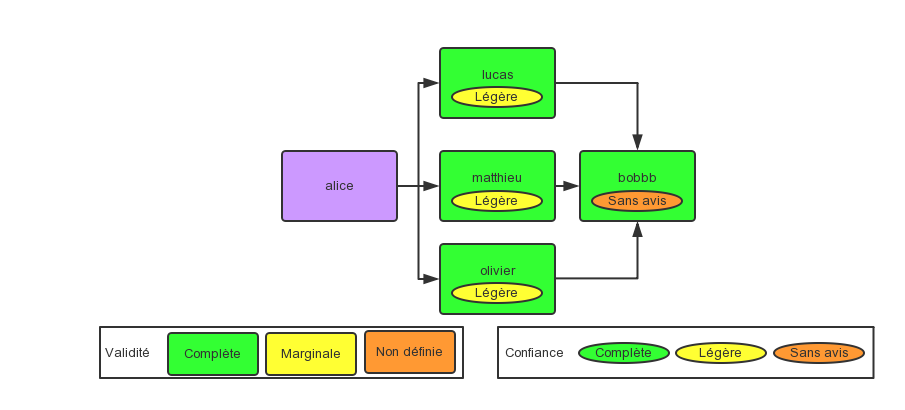
\includegraphics[scale=0.3]{tdcdemoComplete1.png}
\end{frame}
\begin{frame}
  \frametitle{\color{white}Validité Complète}
    \begin{block}{}
      Une clef certifié par Alice avec une confiance complète
      suffit a propager une validité complète sur une clé non certifié par Alice mais
      certifié par la première.
    \end{block}
    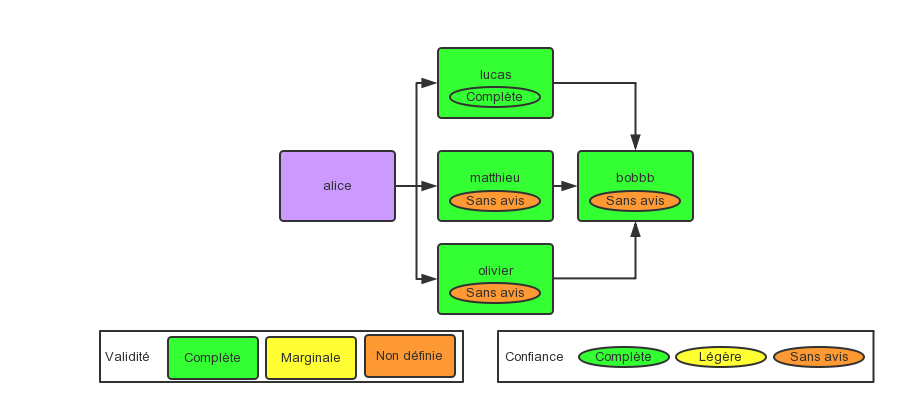
\includegraphics[scale=0.3]{tdcdemoComplete2.png}
\end{frame}

\begin{frame}
  \frametitle{\color{white}GuiPG}
  \begin{block}{Gestion d'un trousseau de clé gpg}
      \begin{itemize}
        \item Création de clé / sous clé.
        \item Suppression de clé principale.
        \item Certification de clé.
        \item Modification de la confiance.
        \item Ajouter un identifiant utilisateur.
        \item Importation / Exportation de clés depuis un fichier.
      \end{itemize}
    \end{block}
    \begin{block}{Opérations cryptographique}
      \begin{itemize}
        \item Chiffrer un fichier, pour plusieurs destinataires de façon anonyme ou non.
        \item Déchiffrer un fichier et vérifier les signatures.
      \end{itemize}
    \end{block}
\end{frame}

\begin{frame}
  \frametitle{\color{white}Attaque}
  \begin{block}{Attaque sur les identifiants de clé}
      \begin{itemize}
        \item Forger une 2\up{nd} pré-image d'une clé sur les 8 derniers caractères de son identifiant.
        %\item Documentation sur les limites de GnuPG.
      \end{itemize}
    \end{block}
  \begin{block}{Lexique}
      \begin{itemize}
        \item Clef PGP = clef RSA encapsulé dans un paquet PGP
        \item Le fingerprint est l'empreinte d'une clef
        \item Le KeyId est l'idenfiant de la clef
      \end{itemize}
    \end{block}
\end{frame}

\begin{frame}
  \frametitle{\color{white}Attaque}
  \begin{block}{ }
  Le but de cette attaque est de trouver une seconde clef possédant le même KeyId que la première. Cette attaque est issue du dépot github de Jameson
  Rollins et Danivel Kahn Gillmor.
  \end{block}
  \begin{block}{Fonctionnement de l'attaque}
      \begin{itemize}
        \item Crée une clef RSA.
        \item Modifie la date de création jusqu'à ce que le haché soit identique à la clef voulu
        \item Fabrique un paquet PGP avec la clef RSA pour qu'il soit importable dans GnuPG
      \end{itemize}
  \end{block}
\end{frame}

\begin{frame}
  \frametitle{\color{white}Les contraintes de l'attaque}
  \begin{block}{Date de création}
      \begin{itemize}
        \item La date de création doit être supérieure à 1970 l'année 0 dans les machines.
        \item La date de création doit être inférieure à la date d'aujourd'hui.
      \end{itemize}
    \end{block}
    \medbreak
    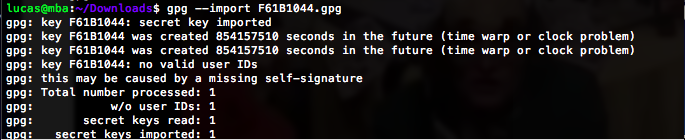
\includegraphics[scale=0.42]{attaque.png}
\end{frame}


\section{Les risques survenus}
  \subsection{Risques organisationnels}
    \begin{frame}
      \frametitle{\color{white}Risques organisationnels}
      \begin{block}{Perte de membres}
        Deux membres ont quitté le projet durant le premier sprint.
      \end{block}
      \begin{block}{Incompatibilité d'emploi du temps}
        Deux membres sont passés en GIL.\\
        Difficultés pour se réunir.
      \end{block}
      \pause
      \begin{exampleblock}{Solutions}
        \begin{itemize}
          \item Mis en place d'un plan d'action
          \item Redéfinition du périmètre du projet
          \item Mise en place d'un créneau hebdomadaire commun.
        \end{itemize}
      \end{exampleblock}
    \end{frame}

  \subsection{Risques techniques}
    \begin{frame}
      \frametitle{\color{white}Maîtrise des outils}
      \begin{block}{Maîtrise des outils}
        Majorité des membres pas assez formée sur les outils utilisé\\
        (git, Qt, C++, gpg)
      \end{block}
      \pause
      \begin{exampleblock}{Solutions}
        \begin{itemize}
          \item Réunion d'installation et de formation aux outils
        \end{itemize}
      \end{exampleblock}
    \end{frame}
    \begin{frame}
      \frametitle{\color{white}Fonctionnement technique de GnuPG}
      \begin{block}{Fonctionnement technique de GnuPG}
        \begin{itemize}
          \item GnuPG utilise directement un tty comme entrée / sortie pour certaine commandes.
          \item Complication de la tâche pour arriver a envoyer et récupérer des données du logiciel.
        \end{itemize}
        
      \end{block}
      \pause
      \begin{exampleblock}{Solutions}
        \begin{itemize}
          \item Inspection du code source de GnuPG et de son comportement
          \item Réalisation d'un pseudo-terminal, a l'aide de l'api système POSIX
        \end{itemize}
      \end{exampleblock}
      \pause
      \begin{alertblock}{Impacts}
        \begin{itemize}
          \item Cette solution, impose un système UNIX \\
                => perte de compatibilité Windows (Exigence optionnelle du besoin)
          \item L'utilisation de bibliothèques nous aurai fait perdre
          la visualisation des commandes gpg
        \end{itemize}
      \end{alertblock}
    \end{frame}

\section{Bilan du projet}
  
  \subsection{Résultats du projet}
  \begin{frame}
    \frametitle{\color{white}Vue globale du projet}
  \begin{tabular}{|l|l|l|}
    \hline
    \multicolumn{1}{|c|}{\cellcolor{gray} \color{white}Catégories} & \multicolumn{1}{|c|}{\cellcolor{gray} \color{white}Livraison} & \multicolumn{1}{|c|}{\cellcolor{gray} \color{white}Livraison initiale} \\
    \hline
    \cellcolor{white}\color{green}Fondation & \multicolumn{1}{|c|}{\cellcolor{white}\color{black}1} & \multicolumn{1}{|c|}{\cellcolor{white}\color{black}1} \\
    \hline
    \cellcolor{white}\color{green}Mécanisme multi-instance & \multicolumn{1}{|c|}{\cellcolor{white}\color{black}1} & \multicolumn{1}{|c|}{\cellcolor{white}\color{black}1} \\    
    \hline
    \cellcolor{white}\color{green}Gestion des profils & \multicolumn{1}{|c|}{\cellcolor{white}\color{black}1} & \multicolumn{1}{|c|}{\cellcolor{white}\color{black}1} \\
    \hline
    \cellcolor{white}\color{yellow}Gestion des clefs & \multicolumn{1}{|c|}{\cellcolor{white}\color{black}2} & \multicolumn{1}{|c|}{\cellcolor{white}\color{black}1} \\
    \hline
    \cellcolor{white}\color{green}Vue des commandes et retours GPG & \multicolumn{1}{|c|}{\cellcolor{white}\color{black}2} & \multicolumn{1}{|c|}{\cellcolor{white}\color{black}1} \\
    \hline
    \cellcolor{white}\color{yellow}Opérations cryptographiques & \multicolumn{1}{|c|}{\cellcolor{white}\color{black}2} & \multicolumn{1}{|c|}{\cellcolor{white}\color{black}2} \\
    \hline
    \cellcolor{white}\color{yellow}\'{E}diteur & \multicolumn{1}{|c|}{\cellcolor{white}\color{black}2} & \multicolumn{1}{|c|}{\cellcolor{white}\color{black}2} \\
    \hline
    \cellcolor{white}\color{red}Attaque & \multicolumn{1}{|c|}{\cellcolor{white}\color{black}2} & \multicolumn{1}{|c|}{\cellcolor{white}\color{black}3} \\
    \hline
    \cellcolor{white}\color{red}\'{E}tude gestion des clefs & \multicolumn{1}{|c|}{\cellcolor{white}\color{black}} & \multicolumn{1}{|c|}{\cellcolor{white}\color{black}1} \\
    \hline
    \cellcolor{white}\color{red}\'{E}tude des opérations cryptographiques & \multicolumn{1}{|c|}{\cellcolor{white}\color{black}} & \multicolumn{1}{|c|}{\cellcolor{white}\color{black}2} \\
    \hline
    \cellcolor{white}\color{red}\'{E}tude gestion de la toile de confiance & \multicolumn{1}{|c|}{\cellcolor{white}\color{black}} & \multicolumn{1}{|c|}{\cellcolor{white}\color{black}2} \\
    \hline
    \cellcolor{white}\color{red}\'{E}tude des limites & \multicolumn{1}{|c|}{\cellcolor{white}\color{black}} & \multicolumn{1}{|c|}{\cellcolor{white}\color{black}3} \\
    \hline
    \cellcolor{white}\color{red}Toile de confiance statique & \multicolumn{1}{|c|}{\cellcolor{white}\color{black}} & \multicolumn{1}{|c|}{\cellcolor{white}\color{black}2} \\
    \hline
    \cellcolor{white}\color{red}Toile dynamique & \multicolumn{1}{|c|}{\cellcolor{white}\color{black}} & \multicolumn{1}{|c|}{\cellcolor{white}\color{black}3} \\
    \hline
  \end{tabular}
\end{frame}

\subsection{Améliorations et rétrospective}
  \begin{frame}
    \frametitle{\color{white}Ce qu'on pourrait améliorer}
    \begin{block}{Axes d'améliorations}
      Améliorations de l'interface GuiPG :
      \begin{itemize}
        \item Affiner la gestion de clé.
        \item Ajouter une visualisation sous forme de graphe de la toile de confiance.
        \item Développer l'éditeur de texte.
        \item Personnaliser l'interface.
      \end{itemize}
      Améliorations de l'attaque :
      \begin{itemize}
        \item Paralléliser le calcul des hashs de la clé sur CPU.
        \item Implanter l'attaque sur carte graphique (OpenCL, CUDA).
      \end{itemize}
    \end{block}
    
  \end{frame}

  \begin{frame}
  \frametitle{\color{white}Si c'était à refaire}
    \begin{block}{Rétrospective}
    Approfondir l'étude de faisabilité lors de la phase d'avant projet.
      \begin{itemize}
        \item Réaliser une prise en main poussée du logiciel gpg.
        \item S'assurer de la compréhension et de la maîtrise des outils de la part de chacun.
        \item Utiliser Python.
      \end{itemize}
    \end{block}


  \end{frame}
